\documentclass[10pt]{beamer}
\definecolor{aliceblue}{rgb}{0.94, 0.97, 1.0}
\setbeamercolor{background canvas}{bg=aliceblue}
\usetheme[progressbar=frametitle]{metropolis}
\usepackage{appendixnumberbeamer}
\usepackage{booktabs}
\usepackage[scale=2]{ccicons}
\usepackage{pgfplots}
\usepgfplotslibrary{dateplot}
\usepackage{xspace}
\usepackage[yyyymmdd,hhmmss]{datetime}
\newcommand{\themename}{\textbf{\textsc{metropolis}}\xspace}




\titlegraphic{
	\begin{picture}(0,49.5)(10,-10)
	
\includegraphics[scale=0.025]{img/logo.png}
	\end{picture}
}

\setbeamertemplate{footline}[frame number]
\logo{
\includegraphics[scale=0.025,keepaspectratio]{img/logo.png}}

\setbeamertemplate{sidebar right}{}
\defbeamertemplate*{footline}{logo-frame number}
{
	\rlap{\raisebox{-6.5ex}[0pt][0pt]{\makebox[\paperwidth]{\insertlogo}}}%
	\hfill%
	\usebeamercolor[fg]{page number in head/foot}%
	\usebeamerfont{page number in head/foot}%
	\insertframenumber\,/\,  \inserttotalframenumber\kern3em\vskip20pt%
}



\title{Netbreak}
\subtitle{Revisione di Progettazione}
\author{
	Dan Serbanoiu\\      
	\and
	Andrea Scalabrin\\  
	\and
	Nicol\`{o} Scapin\\  
	\and
	Alberto Nicol\`{e}\\  
	\and
	Davide Scarparo\\  
	\and
	Marco Casagrande\\   
}
% \date{\today}
\date{\today}

\institute{Universit\`{a} di Padova}
% \titlegraphic{\hfill
\includegraphics[height=1.5cm]{logo.pdf}}

\begin{document}

\maketitle

\begin{frame}{Table of contents}
	\begin{enumerate}
		\item Tecnologie
		\item Design Architetturale
		\item Front-End
		\item Back-End
	\end{enumerate}
\end{frame}

\newpage
\section{Tecnologie}
\subsection{AngularJS}
Per lo sviluppo della parte \textit{Front-End\ped{G}} dell'applicazione si è scelto di usare il \textit{framework\ped{G}} \textit{JavaScript\ped{G}} \textit{AngularJS\ped{G}}, che permette lo sviluppo di applicazioni in singola pagina. Esso consente di utilizzare HTML\ped{G} come linguaggio di template e permette di estenderne la sintassi per esprimere i componenti dell'applicazione in modo chiaro e conciso.

\subsection{Node.js}
La Web app necessita di \textit{node.js\ped{G}} per essere eseguita. Esso permette di realizzare applicazioni Web, come appunto API Market, utilizzando il linguaggio JavaScript, tipicamente client-side, per la scrittura server-side. La caratteristica principale di Node.js risiede nella possibilità che offre di accedere alle risorse del sistema operativo in modalità \textit{event-driven\ped{G}} non sfruttando il classico modello basato su processi o thread concorrenti, utilizzato dai classici web server. In particolare, si utilizzano diversi pacchetti npm dall'ecosistema Node.js quali Http-server e Bower. 

\subsection{MySQL}
MySQL o \textit{Database MySQL\ped{G}} è il più diffuso Relational Database Management system (RDBMS) composto da un client a riga di comando e un server. Entrambi i software sono disponibili sia per sistemi Unix e Unix-like che per Windows; le piattaforme principali di riferimento sono Linux e Oracle Solaris. Il software supporta numerosi applicativi per la corretta gestione dei database ad esso associato, ed è rilasciato con licenza Open Source da Oracle. 


\subsection{Jolie}
\textit{Jolie\ped{G}} è il primo linguaggio esplicitamente orientato ai microservizi. E' un linguaggio open-source utilizzato per lo sviluppo back-end a microservizi di API Market. Ogni microservizio del progetto è stato sviluppato a partire da questo linguaggio e integrato con opportune librerie Java. Jolie infatti supporta nativamente un integrazione con Java, dal quale deriva direttamente. 

\subsection{Java}
 \textit{Java\ped{G}} è un linguaggio di programmazione ad alto livello, orientato agli oggetti e a tipizzazione statica, specificatamente progettato per essere il più possibile indipendente dalla piattaforma di esecuzione. Vista la diffusione di Java e l'integrazione nativa con il linguaggio Jolie, esso si presta per l'integrazione di librerie di terze parti, quali ad esempio controlli JDBC per la connessione ai database. 
 
\subsection{Javascript}
JavaScript è un linguaggio di scripting orientato agli oggetti e agli eventi, comunemente utilizzato nella programmazione Web lato client per la creazione, in siti web e applicazioni web, di effetti dinamici interattivi tramite funzioni di script invocate da eventi innescati a loro volta in vari modi dall'utente sulla pagina web in uso (mouse, tastiera, caricamento della pagina ecc...). Tali funzioni di script possono essere opportunamente inserite in file HTML, in pagine JSP o in appositi file separati con estensione .js poi richiamati nella logica di business.

\subsection{JQuery}
\textit{jQuery\ped{G}} è una libreria JavaScript per applicazioni web. Nasce con l'obiettivo di semplificare la selezione, la manipolazione, la gestione degli eventi e l'animazione di elementi DOM in pagine HTML, nonché implementare funzionalità AJAX. 

\subsection{Bootstrap 3}
\textit{Bootstrap 3\ped{G}} è una raccolta di strumenti per la creazione di siti e applicazioni Web. Essa contiene modelli di progettazione basati su HTML e \textit{CSS\ped{G}}, sia per la tipografia, che per le varie componenti dell’interfaccia, come moduli, così come alcune estensioni opzionali di JavaScript.
\section{Design Architetturale}

\begin{frame}{MVVM}
	\begin{figure}
		\centering
		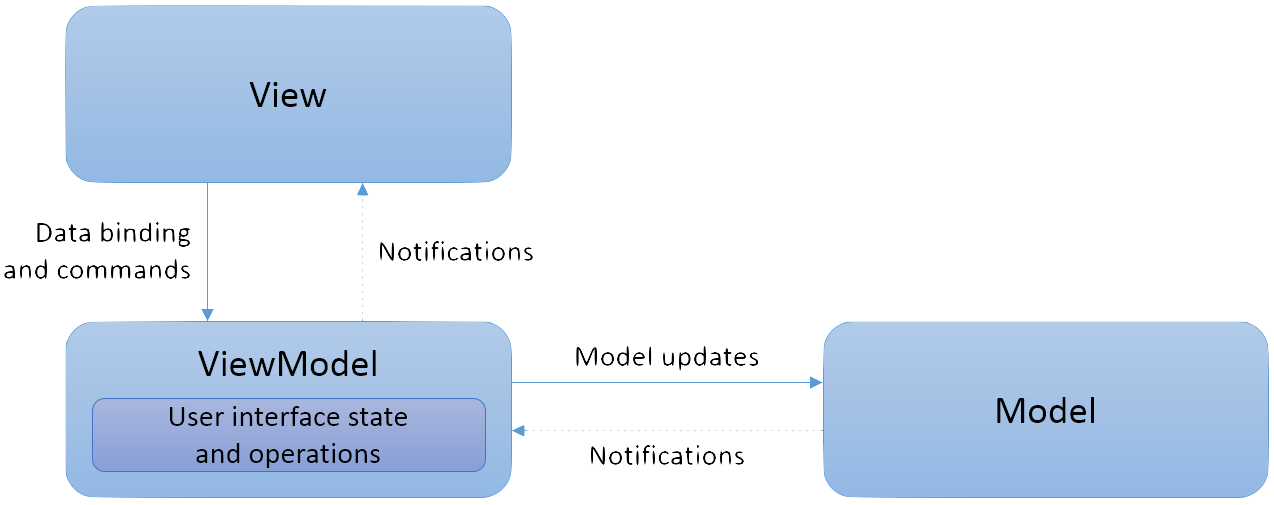
\includegraphics[scale=0.4]{img/mvvm.png}
		\caption{MVVM}
		
	\end{figure}
\end{frame}


\newpage
\section{Packages Front-end}

\subsection{node\_modules}
\begin{itemize}
	\item \textbf{Padre}: FrontEnd;
	
	\item \textbf{Descrizione}: package che raccoglie le librerie esterne di JavaScript, installate tramite \textit{npm} di Node.js, e fornisce le funzionalità necessarie alla parte di front-end dell'applicazione;
	
	\item \textbf{Relazioni d’uso con altri componenti}: questo package si relaziona con i \textit{controllers} presenti nel sub-package \textit{Controllers} del package \textit{App}.
\end{itemize}

\subsection{App}

\begin{figure}[H]
	\centering
	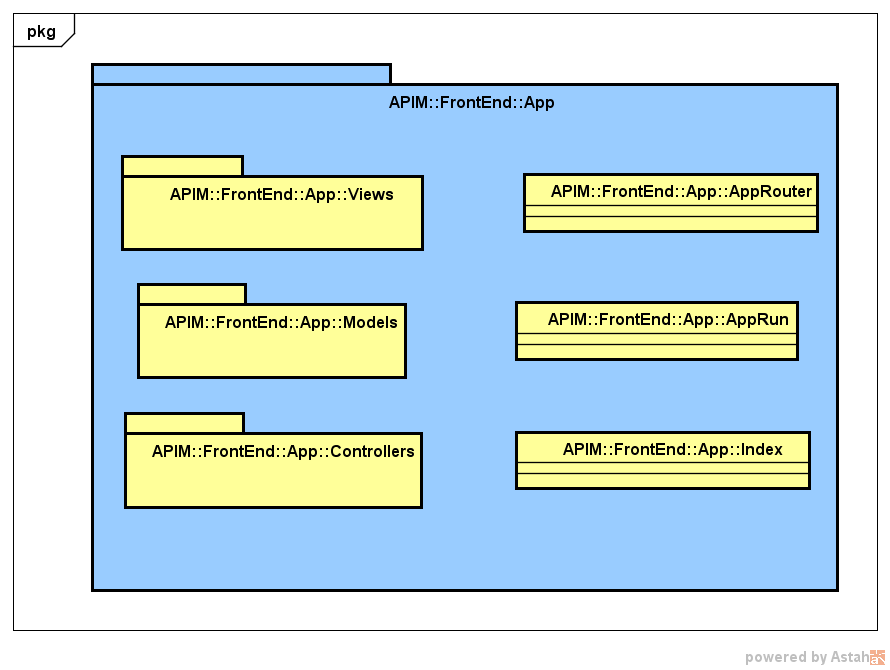
\includegraphics
	[width=0.7\linewidth]
	{UML/DiagrammiPackage/app.png}
	\caption{Package APIM::FrontEnd::App}
\end{figure}

\begin{itemize}
	\item \textbf{Padre}: FrontEnd;
	
	\item \textbf{Descrizione}: package che raccoglie le componenti principali del front-end dell'applicazione web, secondo il pattern architetturale Model-View-Controller (MVC);
	
	\item \textbf{Relazioni d’uso con altri componenti}: questo package si relaziona con le librerie presenti nel sub-package \textit{node\_modules} del package padre;
	
	\item \textbf{Package contenuti}:
	\begin{itemize}
		\item \textbf{\textit{Views}}: package contenente le \textit{views} del front-end dell'applicazione;
		
		\item \textbf{\textit{Models}}: package contenente i \textit{models} del front-end dell'applicazione;
		
		\item \textbf{\textit{Controllers}}: package contenente i \textit{controllers} del front-end dell'applicazione.
	\end{itemize}
	\item \textbf{Classi contenute}:
	\begin{itemize}
		
		\item \textbf{\textit{AppRun}}: classe che istanzia l'applicazione;
		
		\item \textbf{\textit{AppRouter}}: classe che gestisce i routes dell'applicazione;
		
		\item \textbf{\textit{Index}}: view generale dell'applicazione (single page app).
	\end{itemize}
\end{itemize}

\subsubsection{AppRun}

\begin{itemize}
	\item \textbf{Padre}: App;
	
	\item \textbf{Descrizione}: classe che istanzia l'applicazione e che viene utilizzata per indicare le dipendenze tra l'applicazione e i packages esterni.
\end{itemize}

\subsubsection{AppRouter}

\begin{itemize}
	\item \textbf{Padre}: App;
	
	\item \textbf{Descrizione}: classe che gestisce i routes dell'applicazione al fine di associare ad ogni route un controller e una view (associa un URL alle varie view dell'applicazione).
\end{itemize}

\subsubsection{Index}

\begin{itemize}
	\item \textbf{Padre}: App;
	
	\item \textbf{Descrizione}: classe che rappresenta la view generale dell'applicazione e che contiene gli elementi che saranno presenti in ogni pagina dell'applicazione.
\end{itemize}

\subsubsection{Views}

\begin{figure}[H]
	\centering
	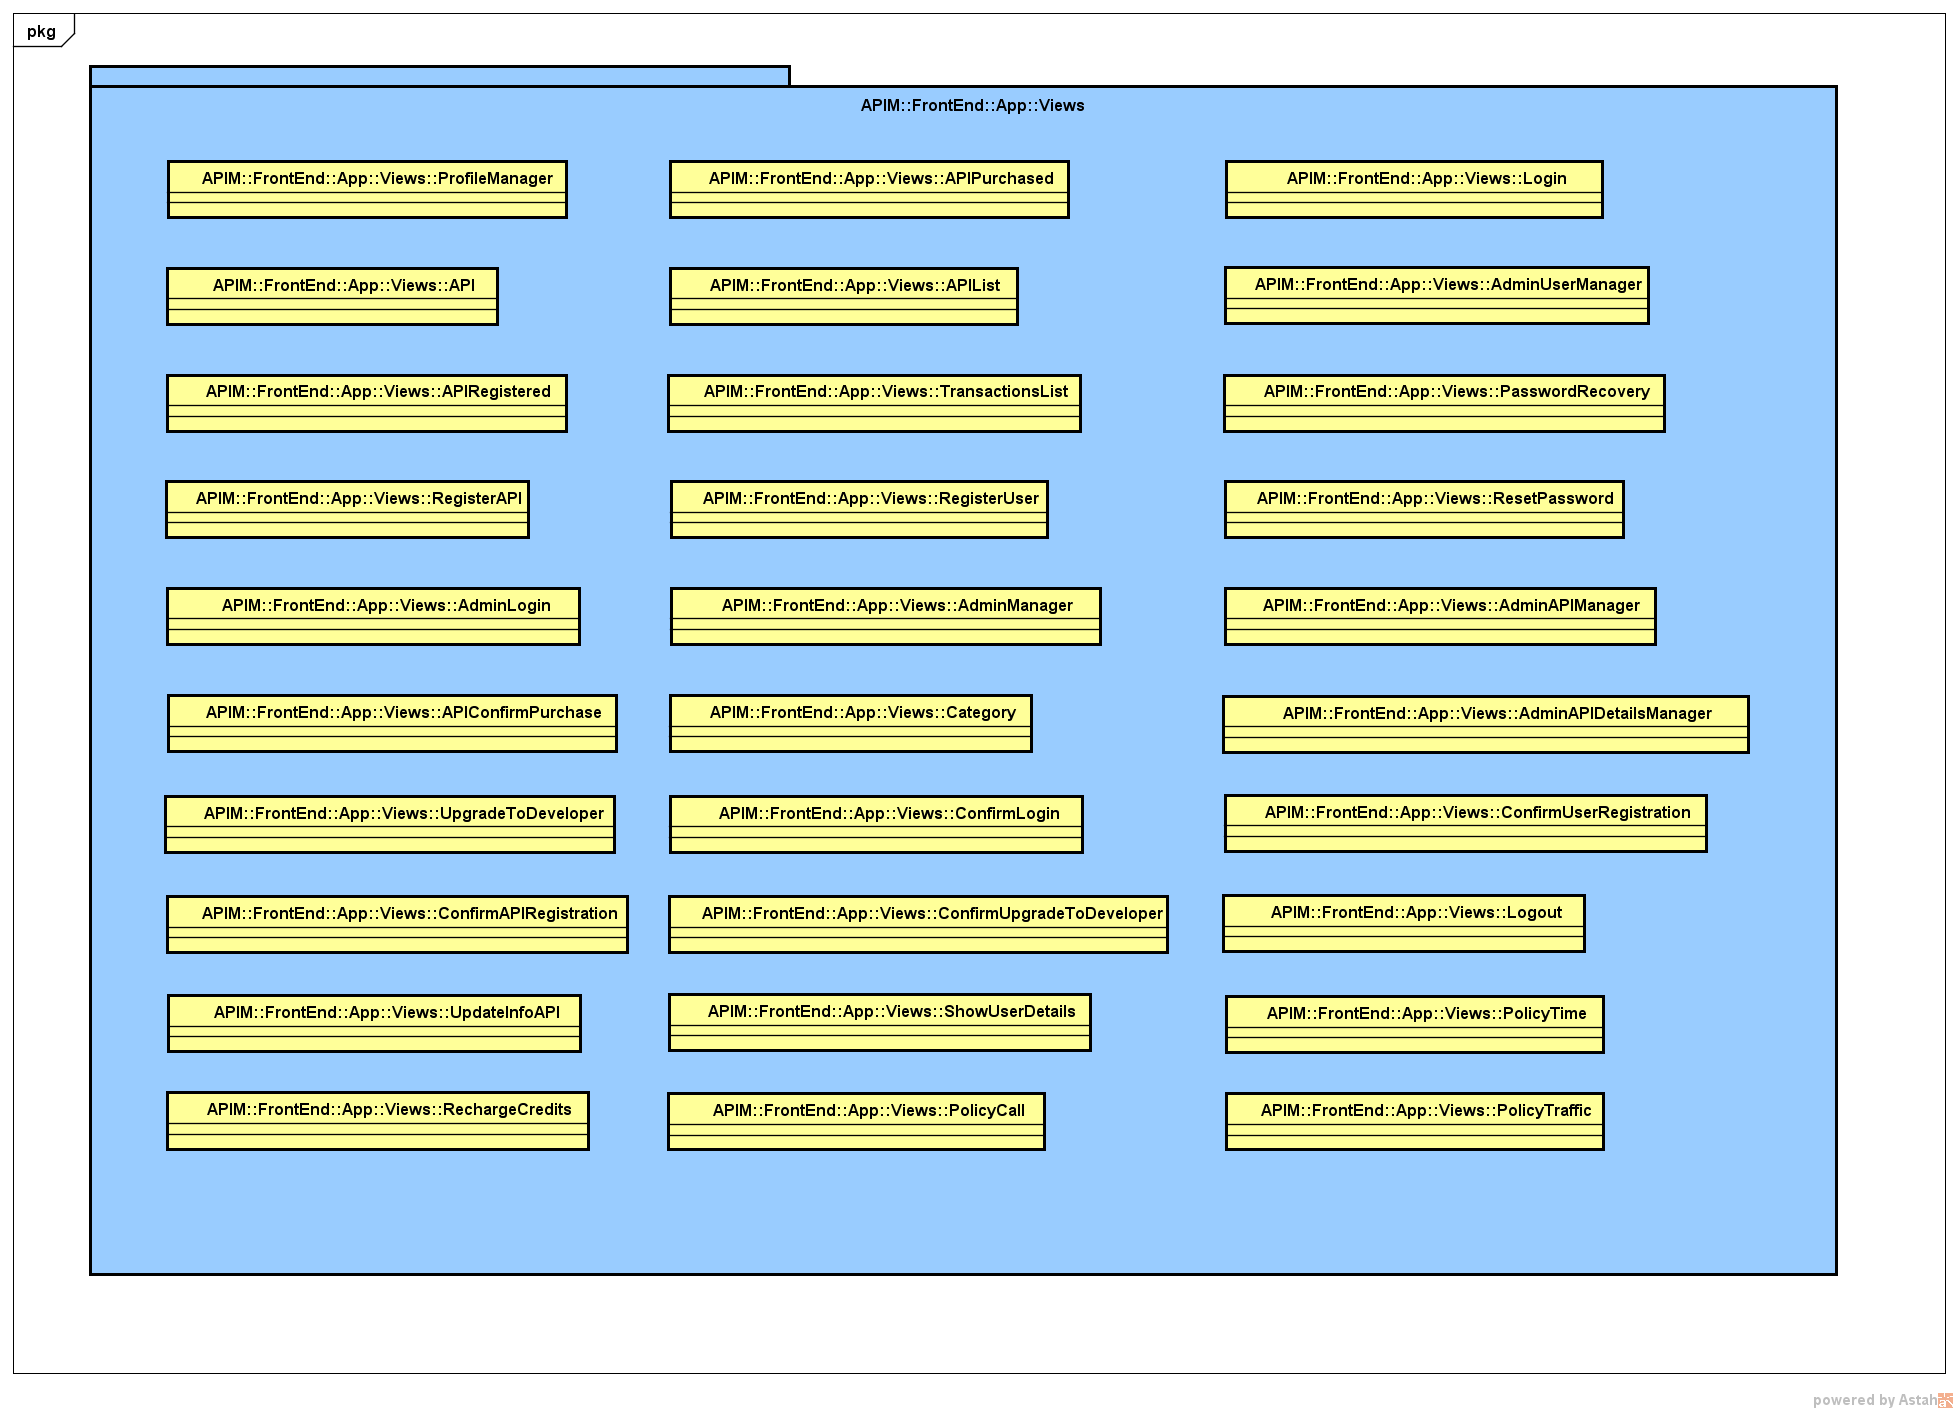
\includegraphics
	[width=0.9\linewidth]
	{UML/DiagrammiPackage/views.png}
	\caption{Package APIM::FrontEnd::App::Views}
\end{figure}

\begin{itemize}
	\item \textbf{Padre}: App;
	
	\item \textbf{Descrizione}: package contenente tutte le classi che rappresentano i vari template HTML per le pagine web dell'applicazione;
	
	\item \textbf{Relazioni d’uso con altri componenti}: questo package si relaziona con i \textit{controllers} presenti nel package \textit{Controllers};
	
	\item \textbf{Classi contenute}:
	\begin{itemize}
		\item \textbf{\textit{RegisterUser}}: view contenente il form dedicato alla registrazione di un utente, il quale può inserire i campi necessari e registrarsi così alla piattaforma. Contiene, inoltre, un link alla pagina di login.\\
		Si relaziona con le seguenti componenti: \textit{UserRegistrationController}.
		
		\item \textbf{\textit{Login}}: view contenente il form necessario affinchè l'utente possa effettuare il login ed autenticarsi al sistema. Contiene, inoltre, un link alla pagina di registrazione e uno alla pagina per il recupero della password.\\
		Si relaziona con le seguenti componenti: \textit{LoginController}.
		
		\item \textbf{\textit{PasswordRecovery}}: view contenente il form dedicato al recupero della password di un utente, il quale può inserire l'indirizzo email e ricevere una nuova password con la quale autenticarsi al sistema. Contiene, inoltre, un link alla pagina di login.\\
		Si relaziona con le seguenti componenti: \textit{PasswordRecoveryController}.
		
		\item \textbf{\textit{API}}: view contenente i risultati della ricerca effettuata, che permette di selezionare un risultato presente al suo interno.\\
		Si relaziona con le seguenti componenti: \textit{APIController}.
		
		\item \textbf{\textit{ProfileManager}}: view contenente le informazioni del profilo personale di un utente registrato. Contiene, inoltre, l'informazione relativa al saldo del proprio conto virtuale.\\
		Si relaziona con le seguenti componenti: \textit{ProfileManagerController}.
		
		\item \textbf{\textit{ResetPassword}}: view contenente il form dedicato al cambio di password di un utente autenticato, il quale può inserire la nuova password che intende utilizzare per i futuri login al sistema.\\
		Si relaziona con le seguenti componenti: \textit{ResetPasswordController}.
		
		\item \textbf{\textit{RegisterAPI}}: view contenente il form per l'inserimento di una API da parte di un utente sviluppatore. Lo sviluppatore può inserire tutti i dati relativi al microservizio che intende esporre sul marketplace.\\
		Si relaziona con le seguenti componenti: \textit{APIRegistrationController}.
		
		\item \textbf{\textit{PolicyCall}}: view contenente le informazioni relative alla policy per chiamate.\\
		Si relaziona con le seguenti componenti: \textit{PolicyCallController}.
		
		\item \textbf{\textit{PolicyTime}}: view contenente le informazioni relative alla policy per tempo.\\
		Si relaziona con le seguenti componenti: \textit{PolicyTimeController}.
		
		\item \textbf{\textit{PolicyTraffic}}: view contenente le informazioni relative alla policy per traffico dati.\\
		Si relaziona con le seguenti componenti: \textit{PolicyTrafficController}.
		
		\item \textbf{\textit{APIRegistered}}: view contenente le informazioni di una API registrata sulla piattaforma.\\
		Si relaziona con le seguenti componenti: \textit{APIRegisteredController}.
		
		\item \textbf{\textit{APIPurchased}}: view contenente le informazioni delle API acquistate da un cliente della piattaforma \progetto.\\
		Si relaziona con le seguenti componenti: \textit{APIPurchasedController}.
		
		\item \textbf{\textit{APIList}}: view contenente l'elenco delle API disponibili sul marketplace \progetto.\\
		Si relaziona con le seguenti componenti: \textit{APIListController}.
		
		\item \textbf{\textit{TransactionsList}}: view contenente l'elenco delle transazioni effettuate da un utente sul marketplace \progetto.\\
		Si relaziona con le seguenti componenti: \textit{TransactionsListController}.
		
		\item \textbf{\textit{APIConfirmPurchase}}: view contenente la conferma di un acquisto di una API.\\
		Si relaziona con le seguenti componenti: \textit{APIConfirmPurchaseController}.
		
		\item \textbf{\textit{AdminManager}}: view contenente le operazioni per la gestione del profilo amministratore \progetto.\\
		Si relaziona con le seguenti componenti: \textit{AdminManagerController}.
		
		\item \textbf{\textit{Category}}: view contenente l'elenco delle categoria nell'\progetto.\\
		Si relaziona con le seguenti componenti: \textit{CategoryController}.
		
		\item \textbf{\textit{ConfirmUpgradeToDeveloper}}: view contenente la conferma dell'upgrade di un utente a sviluppatore nell'\progetto.\\
		Si relaziona con le seguenti componenti: \textit{ConfirmUpgradeToDeveloperController}.
		
		\item \textbf{\textit{ConfirmLogin}}: view contenente la conferma di login all'\progetto.\\
		Si relaziona con le seguenti componenti: \textit{ConfirmLoginController}.
		
		\item \textbf{\textit{ConfirmUserRegistration}}: view contenente la conferma di registrazione all'\progetto.\\
		Si relaziona con le seguenti componenti: \textit{ConfirmUserRegistrationController}.
		
		\item \textbf{\textit{ConfirmAPIRegistration}}: view contenente la conferma di registrazione di una API all'\progetto.\\
		Si relaziona con le seguenti componenti: \textit{ConfirmAPIRegistrationController}.
		
		\item \textbf{\textit{UpgradeToDeveloper}}: view contenente il modulo per diventare sviluppatore all'interno dell'\progetto.\\
		Si relaziona con le seguenti componenti: \textit{UpgradeToDeveloperController}.
		
		\item \textbf{\textit{AdminAPIManager}}: view contenente le operazioni dell'amministratore sulle API dell'\progetto.\\
		Si relaziona con le seguenti componenti: \textit{AdminAPIManagerController}.
		
		\item \textbf{\textit{AdminAPIDetailsManager}}: view contenente le statistiche di una API dell'\progetto.\\
		Si relaziona con le seguenti componenti: \textit{AdminAPIDetailsManagerController}.
		
		\item \textbf{\textit{AdminUserManager}}: view contenente le operazioni di un ammistratore sugli utenti dell'\progetto.\\
		Si relaziona con le seguenti componenti: \textit{AdminUserManagerController}.
		
		\item \textbf{\textit{AdminLogin}}: view contenente il form necessario affinchè l'amministratore possa effettuare il login ed autenticarsi al sistema.\\
		Si relaziona con le seguenti componenti: \textit{AdminLoginController}.
		
		\item \textbf{\textit{Logout}}: view contenente la conferma di logout dall'\progetto.\\
		Si relaziona con le seguenti componenti: \textit{LogoutController}.
		
		\item \textbf{\textit{UpdateInfoAPI}}: view contenente il form dedicato modifica delle informazioni di una API presente nel marketplace \progetto.\\
		Si relaziona con le seguenti componenti: \textit{UpdateInfoAPIController}.
		
		\item \textbf{\textit{RechargeCredits}}: view contenente la possibilità di scegliere quanti crediti ricaricare sul conto personale tra i tagli disponibili.\\
		Si relaziona con le seguenti componenti: \textit{RechargeCreditsController}.
		
		item \textbf{\textit{ShowUserDetalis}}: view contenente le informazioni personali di un utente visualizzabili da altri fruitori del marketplace \progetto.\\
		Si relaziona con le seguenti componenti: \textit{ShowUserDetalisController}.
		
		\item \textbf{\textit{AdminModeration}}: view contenente il form dedicato alla moderazione di un utente o di una API/microservizio da parte di un amministratore della piattaforma \progetto.\\
		Si relaziona con le seguenti componenti: \textit{AdminModerationController}.
	\end{itemize}
\end{itemize}

\subsubsection{Models}

\begin{figure}[H]
	\centering
	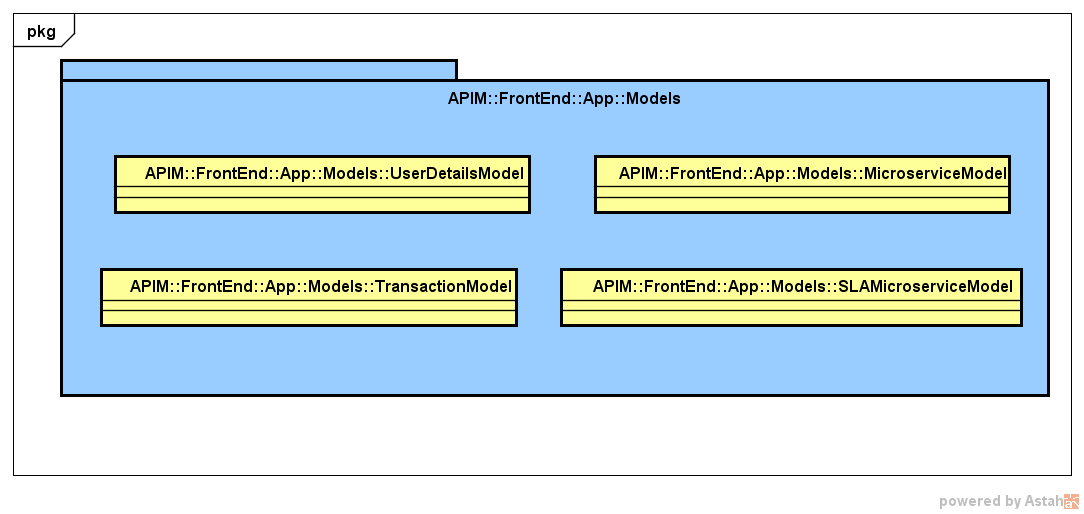
\includegraphics
	[width=0.7\linewidth]
	{UML/DiagrammiPackage/Models.png}
	\caption{Package APIM::FrontEnd::App::Models}
\end{figure}

\begin{itemize}
	\item \textbf{Padre}: App;
	
	\item \textbf{Descrizione}: package che contiene le classi che definiscono la business logic dell'applicazione;
	
	\item \textbf{Relazioni d’uso con altri componenti}: questo package si relaziona con il package \textit{Controllers};
	
	\item \textbf{Classi contenute}:
	\begin{itemize}
		\item \textbf{\textit{UserDetailsModel}}: classe che rappresenta un utente e che contiene tutte le informazioni necessarie alla presentazione del contenuto di un utente, sia nella visualizzazione che nella gestione di un profilo.\\
		Si relaziona con le seguenti componenti: \textit{LoginController}, \textit{APIController}, \textit{ProfileManagerController}, \textit{ResetPasswordController}, \textit{PasswordRecoveryController}.
		
		\item \textbf{\textit{MicroserviceModel}}: classe che rappresenta un microservizio e che contiene tutte le informazioni necessarie alla presentazione del contenuto di un microservizio, sia nella visualizzazione che nella gestione.\\
		Si relaziona con le seguenti componenti: \textit{APIRegiteredController}, \textit{APIRegistrationController}, \textit{PolicyCallController}, \textit{PolicyTimeController}, \textit{PolicyTrafficController}, \textit{APIPurchasedController}, \textit{APIListController}.
		
		\item \textbf{\textit{TransactionModel}}:  classe che rappresenta una transazione avvenuta e che contiene tutte le informazioni necessarie alla presentazione del contenuto di una transazione, sia nella visualizzazione che nella gestione.\\
		Si relaziona con le seguenti componenti: \textit{TransactionsListController}, \textit{APIPurchasedController}.
		
		\item \textbf{\textit{SLAMicroserviceModel}}:  classe che rappresenta la SLA di un microservizio e che contiene tutte le informazioni necessarie alla presentazione del contenuto di SLA di un microservizio, sia nella visualizzazione che nella gestione.\\
		Si relaziona con le seguenti componenti: \textit{PolicyCallController}, \textit{PolicyTimeController}, \textit{PolicyTrafficController}, \textit{APIRegistrationController}.
	\end{itemize}
\end{itemize}

\subsubsection{Controllers}

\begin{figure}[H]
	\centering
	\includegraphics
	[width=0.9\linewidth]
	{UML/DiagrammiPackage/controllers.png}
	\caption{Package APIM::FrontEnd::App::Controllers}
\end{figure}

\begin{itemize}
	\item \textbf{Padre}: App;
	
	\item \textbf{Descrizione}: package che contiene i \textit{controllers} individuati per la parte front-end
	dell'applicazione, i quali consentono la gestione delle azioni utente dell'applicazione web;
	
	\item \textbf{Relazioni d’uso con altri componenti}: questo package si relaziona con i package \textit{Views} e \textit{Models}.
	
	\item \textbf{Classi contenute}:
	\begin{itemize}
		
		\item \textbf{\textit{RegisterUserController}}: classe che permette di gestire la registrazione di un utente al sistema, fornendone le funzionalità preposte.\\
		Si relaziona con le seguenti componenti: \textit{RegisterUser}.
		
		\item \textbf{\textit{LoginController}}: classe che permette di gestire il login di un utente alla piattaforma \progetto, fornendo le funzionalità di autenticazione al sistema, compresa la gestione di	situazioni di errore di autenticazione.\\
		Si relaziona con le seguenti componenti: \textit{UserDetailsModel}, \textit{Login}.
		
		\item \textbf{\textit{PasswordRecoveryController}}: classe che permette di gestire il ripristino della password dimenticata da un utente, fornendo tutte le funzionalità per il recupero della password dopo aver verificato l'identità dell'utente.\\
		Si relaziona con le seguenti componenti: \textit{UserDetailsModel}, \textit{PasswordRecovery}.
		
		\item \textbf{\textit{APIController}}: classe che permette di gestire la ricerca di microservizi all'interno del marketplace \progetto, fornendo all'utente le funzionalità di ricerca tramite categorie e keywords per sviluppatori e microservizi.\\
		Si relaziona con le seguenti componenti: \textit{API}.
		
		\item \textbf{\textit{ProfileManagerController}}: classe che permette di gestire il profilo personale di un utente, fornendo le funzionalità all'utente per poter modificare i propri dati.\\
		Si relaziona con le seguenti componenti: \textit{UserDetailsModel}, \textit{ProfileManager}.
		
		\item \textbf{\textit{ResetPasswordController}}: classe che permette di gestire il cambio password di un utente autenticato al sistema, fornendo le funzionalità per il salvataggio di una nuova password.\\
		Si relaziona con le seguenti componenti: \textit{UserDetailsModel}, \textit{ResetPassword}.
		
		\item \textbf{\textit{RegisterAPIController}}: classe che permette di gestire l'inserimento di una API, fornendo tutte le funzionalità atte alla corretta esposizione di un microservizio di uno sviluppatore, utente della piattaforma \progetto.\\
		Si relaziona con le seguenti componenti: \textit{MicroserviceModel}, \textit{RegisterAPI}.
		
		\item \textbf{\textit{PolicyCallController}}: classe che permette di gestire le policy di vendita dei microservizi per chiamate.\\
		Si relaziona con le seguenti componenti: \textit{PolicyCall}, \textit{SLAMicroserviceModel}.
		
		\item \textbf{\textit{PolicyTimeController}}: classe che permette di gestire le policy di vendita dei microservizi per tempo.\\
		Si relaziona con le seguenti componenti: \textit{PolicyTime}, \textit{SLAMicroserviceModel}.
		
		\item \textbf{\textit{PolicyTrafficController}}: classe che permette di gestire le policy di vendita dei microservizi per traffico dati.\\
		Si relaziona con le seguenti componenti: \textit{PolicyTraffic}, \textit{SLAMicroserviceModel}.
		
		\item \textbf{\textit{APIRegisteredController}}: classe che permette di gestire le informazioni di una API precedentemente inserita.\\
		Si relaziona con le seguenti componenti: \textit{MicroserviceModel}, \textit{APIRegistered}.
		
		\item \textbf{\textit{APIPurchasedController}}: classe che permette di gestire l'acquisto e le relative informazioni di una API, fornendo l'API Key per l'utilizzo del cliente.\\
		Si relaziona con le seguenti componenti: \textit{APIPurchased}, \textit{MicroserviceModel}, \textit{TransactionModel}.
		
		\item \textbf{\textit{APIListController}}: classe che permette di gestire l'elenco dei microservizi presenti sul marketplace \progetto.\\
		Si relaziona con le seguenti componenti: \textit{APIList}, \textit{MicroserviceModel}.
		
		\item \textbf{\textit{TransactionsListController}}: classe che permette di gestire lo storico delle transazioni di un utente del marketplace \progetto.\\
		Si relaziona con le seguenti componenti: \textit{TransactionsList}, \textit{TransactionsModel}.
		
		\item \textbf{\textit{AdminManagerController}}: classe che permette di gestire il profilo di un amministratore della piattaforma \progetto, fornendo le funzionalità per poter modificare i propri dati e moderare utenti ed API.\\
		Si relaziona con le seguenti componenti: \textit{AdminManager}.
		%----------------------
		
		\item \textbf{\textit{CategoryController}}: classe che permette di gestire l'elenco delle categoria nell'\progetto.\\
		Si relaziona con le seguenti componenti: \textit{Category}.
		
		\item \textbf{\textit{ConfirmUpgradeToDeveloperController}}: classe che permette di gestire la conferma dell'upgrade di un utente a sviluppatore nell'\progetto.\\
		Si relaziona con le seguenti componenti: \textit{ConfirmUpgradeToDeveloper}.
		
		\item \textbf{\textit{ConfirmLoginController}}: classe che permette di gestire la conferma di login all'\progetto.\\
		Si relaziona con le seguenti componenti: \textit{ConfirmLogin}.
		
		\item \textbf{\textit{ConfirmUserRegistrationController}}: classe che permette di gestire la conferma di registrazione all'\progetto.\\
		Si relaziona con le seguenti componenti: \textit{ConfirmUserRegistration}.
		
		\item \textbf{\textit{ConfirmAPIRegistrationController}}: classe che permette di gestire la conferma di registrazione di una API all'\progetto.\\
		Si relaziona con le seguenti componenti: \textit{ConfirmAPIRegistration}.
		
		\item \textbf{\textit{UpgradeToDeveloperController}}: classe che permette di gestire il modulo per diventare sviluppatore all'interno dell'\progetto.\\
		Si relaziona con le seguenti componenti: \textit{UpgradeToDeveloper}.
		
		\item \textbf{\textit{AdminAPIManagerController}}: classe che permette di gestire le operazioni dell'amministratore sulle API dell'\progetto.\\
		Si relaziona con le seguenti componenti: \textit{AdminAPIManager}.
		
		\item \textbf{\textit{AdminAPIDetailsManagerController}}: classe che permette di gestire le statistiche di una API dell'\progetto.\\
		Si relaziona con le seguenti componenti: \textit{AdminAPIDetailsManager}.
		
		\item \textbf{\textit{AdminUserManagerController}}: classe che permette di gestire le operazioni di un ammistratore sugli utenti dell'\progetto.\\
		Si relaziona con le seguenti componenti: \textit{AdminUserManager}.
		
		\item \textbf{\textit{AdminLoginController}}: classe che permette di gestire il form necessario affinchè l'amministratore possa effettuare il login ed autenticarsi al sistema.\\
		Si relaziona con le seguenti componenti: \textit{AdminLogin}.
		
		\item \textbf{\textit{LogoutController}}: classe che permette di gestire la conferma di logout dall'\progetto.\\
		Si relaziona con le seguenti componenti: \textit{Logout}.
		
		\item \textbf{\textit{UpdateInfoAPIController}}: classe che permette di gestire il form dedicato modifica delle informazioni di una API presente nel marketplace \progetto.\\
		Si relaziona con le seguenti componenti: \textit{UpdateInfoAPI}.
		
		\item \textbf{\textit{RechargeCreditsController}}: classe che permette di gestire la possibilità di scegliere quanti crediti ricaricare sul conto personale tra i tagli disponibili.\\
		Si relaziona con le seguenti componenti: \textit{RechargeCredits}.
		
		\item \textbf{\textit{ShowUserDetalisController}}: classe che permette di gestire le informazioni personali di un utente visualizzabili da altri fruitori del marketplace \progetto.\\
		Si relaziona con le seguenti componenti: \textit{ShowUserDetalis}
		
		
		%---------------------
		
		\item \textbf{\textit{AdminModerationController}}: classe che permette di gestire la moderazione di un utente (cliente o sviluppatore che sia) e di API, fornendo le funzionalità per la sospensione e rimozione.\\
		Si relaziona con le seguenti componenti: \textit{AdminModeration}.
		
	\end{itemize}
\end{itemize}
\newpage
\subsection{Back-end}

Nella parte back-end sono presenti i package \textit{Gateway} e \textit{Services} strutturati secondo un'architettura a microservizi, i quali hanno una dipendenza verso l'interfaccia \textit{serviceInteractionHandler}.

\begin{figure}[H]
	\centering
	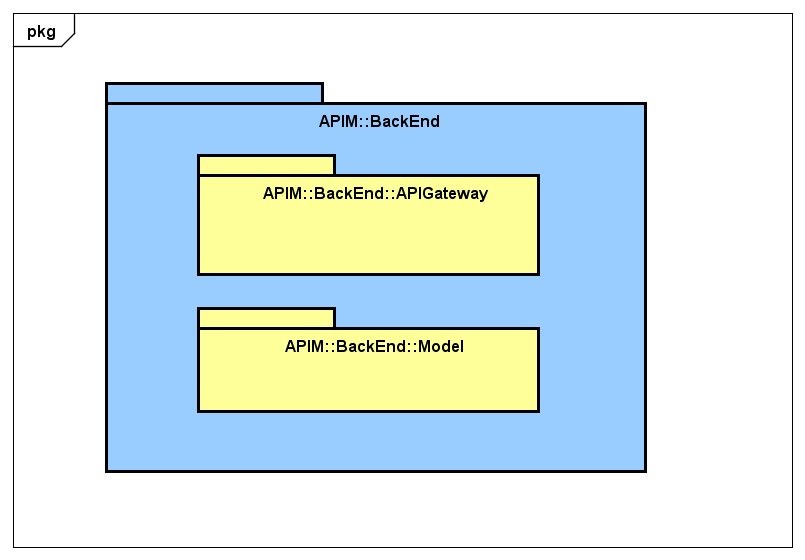
\includegraphics
	[width=0.7\linewidth]
	{UML/DiagrammiPackage/BackEnd.png}
	\caption{Package APIM::BackEnd}
\end{figure}

\begin{itemize}
	\item \textbf{Padre}: APIM;
	
	\item \textbf{Descrizione}: package contenente le componenti del back-end dell'applicazione;
	
	\item \textbf{Package contenuti}:
	\begin{itemize}
		\item \textbf{\textit{Gateway}}: package contenente le classi e le interfacce per il funzionamento dell'API Gateway;
		
		\item \textbf{\textit{Services}}: package contenente tutti i microservizi per le comunicazioni con i database.
	\end{itemize}
	\item \textbf{Classi contenute}:
		\begin{itemize}
			\item \textbf{\textit{serviceInteractionHandler}}: interfaccia per la gestione delle comunicazioni dell'API Gateway e dei \textit{services}.
		\end{itemize}
\end{itemize}

\subsubsection{Gateway}
\begin{figure}[H]
	\centering
	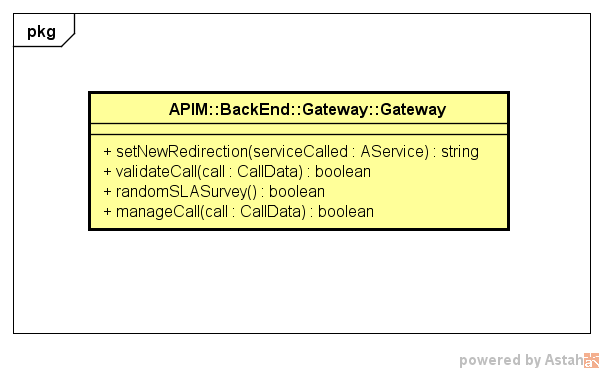
\includegraphics
	[width=0.7\linewidth]
	{UML/DiagrammiPackage/gateway.png}
	\caption{Package APIM::BackEnd::Gateway}
\end{figure}

\begin{itemize}
	\item \textbf{Padre}: BackEnd;
	
	\item \textbf{Descrizione}: package contenente la componente principale del lato back-end. Pur essendo integrato nella sistema, è un modulo che svolge funzioni separate alla piattaforma vera e propria: infatti, l'API Gateway si occupa di controllare e reindirizzare le chiamate effettuate dai clienti ai microservizi (prodotti) inseriti nel marketplace \progetto, verificandone la validità (credenziali, chiave) e monitorandone l'uso (SLA, utilizzi rimanenti).
	
	\item \textbf{Relazioni d'uso con altri componenti}: la classe \textit{Gateway} comunica con le classi contenute all'interno del package \textit{Services}. Inoltre, necessita delle interfacce contenute nel package \textit{Interfaces} e crea le sessioni \textit{couriers} Jolie, archiviandole nel package \textit{Couriers}.
	
	\item \textbf{Package contenuti}:
	\begin{itemize}
		\item \textbf{\textit{Couriers}}: package contenente l'archivio delle sessioni couriers dei microservizi Jolie. Le sessioni couriers vengono create dal gateway ed utilizzate da \textit{serviceinteractionhandler}. Inoltr, forniscono i dati necessari al funzionamento del package \textit{Interfaces}.\\
		Le sessioni couriers permettono l'overloading dei messaggi inviati nelle chiamate dei microservizi al gateway, così da allegare alla richiesta le informazioni per raggiungere il microservizio desiderato.
		
		\item \textbf{\textit{Interfaces}}: package contenente le interfacce necessarie al funzionamento dell'API Gateway. Si occupa dei dati riguardanti le chiamate ai microservizi, in particolar modo, il tipo di operazione richiesta e le informazioni riguardanti l'interfaccia del microservizio target.
	\end{itemize}
	\item \textbf{Classi contenute}:
		\begin{itemize}
			\item \textbf{\textit{Gateway}}: classe che rappresenta la struttura dell'API Gateway della piattaforma \progetto.
		\end{itemize}
\end{itemize}

\subsubsection{Services}
Tale package contiene tutti i servizi appartenenti al lato back-end della piattaforma, eccezion fatta per il gateway già descritto nella sezione soprastante. \textit{Services} contiene tutte le classi di comunicazione con i database che permetteranno il corretto funzionamento dell'applicazione.

\begin{figure}[H]
	\centering
	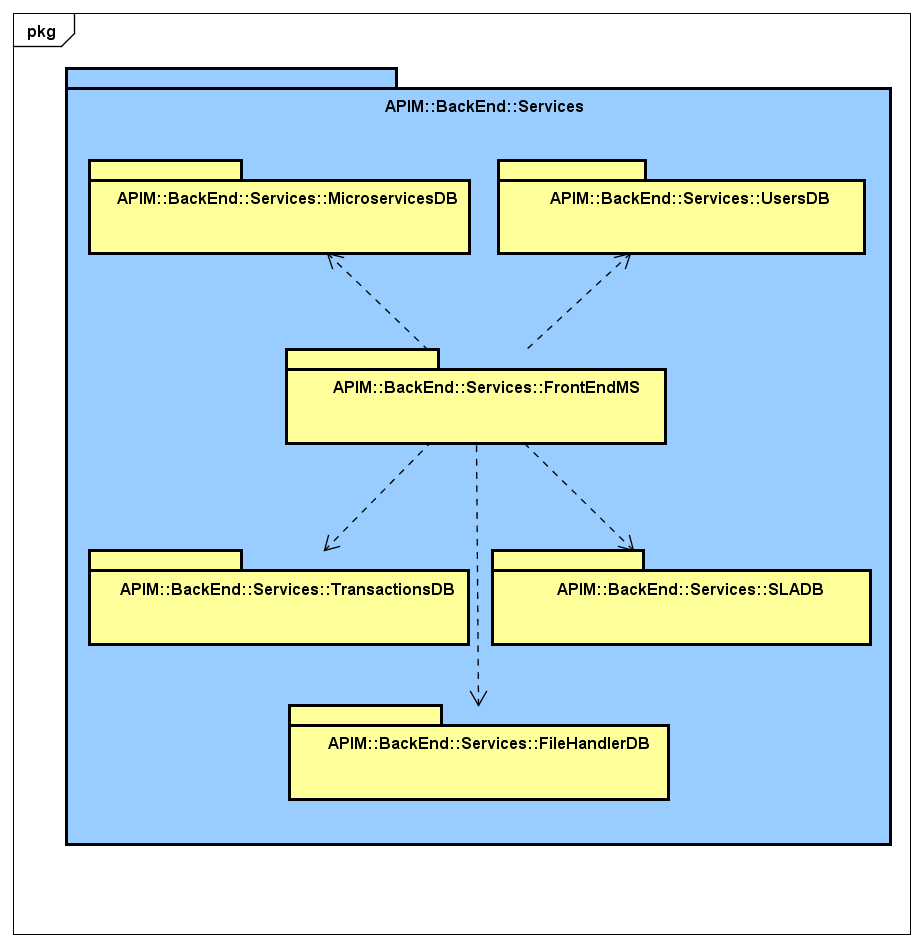
\includegraphics
	[width=0.7\linewidth]
	{UML/DiagrammiPackage/services.png}
	\caption{Package APIM::BackEnd::Services}
\end{figure}

\begin{itemize}
	\item \textbf{Padre}: BackEnd;
	
	\item \textbf{Descrizione}: package che contiene tutti i package relativi ai microservizi del back-end dell'applicazione;
	
	\item \textbf{Relazioni d'uso con altri componenti}: questo package si relaziona con l'API Gateway;
	
	\item \textbf{Package contenuti}:
	\begin{itemize}
		\item \textbf{\textit{UsersDB}}: package contenente le classi che permettono la comunicazione con il database relativo agli utenti del sistema;
		
		\item \textbf{\textit{MicroservicesDB}}: package contenente le classi che permettono la comunicazione con il database relativo ai microservizi registrati sulla piattaforma;
		
		\item \textbf{\textit{TransactionsDB}}: package contenente le classi che permettono la comunicazione con il database relativo alle transazioni degli utenti del sistema;
		
		\item \textbf{\textit{SLADB}}: package contenente le classi che permettono la comunicazione con il database relativo alle informazioni di SLA dei microservizi utilizzati tramite l'API Gateway della piattaforma \progetto;
		
		\item \textbf{\textit{FileHandlerDB}}: package contenente le classi che permettono la gestione dei file;
		
		\item \textbf{\textit{FrontEndMS}}: package contenente le classi che si occupano delle operazioni più complesse, quali l'accesso a più di un database.
	\end{itemize}
\end{itemize}

\paragraph{UsersDB}

\begin{figure}[H]
	\centering
	\includegraphics
	[width=0.7\linewidth]
	{UML/DiagrammiPackage/Users_db.png}
	\caption{Package APIM::BackEnd::Services::UsersDB}
\end{figure}

\begin{itemize}
	\item \textbf{Padre}: Services;
	
	\item \textbf{Descrizione}: package che contiene le classi di comunicazione con il database dell'applicazione relativo alle informazioni (anagrafiche e personali) degli utenti (admin, clienti, sviluppatori) del sistema;
	
	\item \textbf{Relazioni d'uso con altri componenti}: questo package si relaziona con il sub-package \textit{FrontEndMS} del package padre, fornendogli i dati che esso richiede riguardo alle operazioni con il database delle informazioni degli utenti;
	
	\item \textbf{Classi contenute}:
		\begin{itemize}
			\item \textbf{\textit{Users\_dbInterface}}: interfaccia che raccoglie tutte le \textit{operation} riguardanti il database degli utenti;
			
			\item \textbf{\textit{Users\_db}}: classe che implementa l'interfaccia \textit{Users\_dbInterface}.
		\end{itemize}
\end{itemize}

\paragraph{MicroservicesDB}

\begin{figure}[H]
	\centering
	\includegraphics
	[width=0.7\linewidth]
	{UML/DiagrammiPackage/MicroservicesDB.png}
	\caption{Package APIM::BackEnd::Services::MicroservicesDB}
\end{figure}

\begin{itemize}
	\item \textbf{Padre}: Services;
	
	\item \textbf{Descrizione}: package che contiene le classi di comunicazione con il database dell'applicazione relativo ai microservizi registrati nella piattaforma;
	
	\item \textbf{Relazioni d'uso con altri componenti}: questo package si relaziona con il package \textit{FrontendMS}, fornendogli i dati che esso richiede riguardo alle operazioni con il database delle informazioni dei microservizi.\\
	Inoltre, comunica con il Gateway per permettere l'identificazione e l'utilizzo dei microservizi, e garantire correttezza, efficienza e validità delle chiamate;
	
	\item \textbf{Classi contenute}:
	\begin{itemize}
		\item \textbf{\textit{Microservices\_dbInterface}}: interfaccia che raccoglie tutte le \textit{operation} riguardanti il database dei microservizi;
		
		\item \textbf{\textit{Microservices\_db}}: classe che implementa le interfacce \textit{Microservices\_dbInterface} e \textit{serviceInteractionHandler}.
	\end{itemize}
\end{itemize}

\paragraph{TransactionsDB}

\begin{figure}[H]
	\centering
	\includegraphics
	[width=0.7\linewidth]
	{UML/DiagrammiPackage/Transactions_db.png}
	\caption{Package APIM::BackEnd::Services::TransactionsDB}
\end{figure}

\begin{itemize}
	\item \textbf{Padre}: Services;
	
	\item \textbf{Descrizione}: package che contiene le classi di comunicazione con il database dell'applicazione che si occupa di immagazzinare i dati sulle transazioni;
	
	\item \textbf{Relazioni d'uso con altri componenti}: questo package si relaziona con il package \textit{FrontendMS}, fornendogli i dati che esso richiede riguardo alle operazioni con il database delle informazioni delle transazioni.\\
	Comunica inoltre con il Gateway per verificare la validità delle API Key e/o aggiornare i dati relativi (usi residui della chiave) alle chiamate ai microservizi effettuate;
	
	\item \textbf{Classi contenute}:
	\begin{itemize}
		\item \textbf{\textit{Transactions\_dbInterface}}: interfaccia che raccoglie tutte le \textit{operation} riguardanti il database delle transazioni;
		
		\item \textbf{\textit{Transactions\_db}}: classe che implementa l'interfaccia \textit{Transactions\_dbInterface}.
	\end{itemize}
\end{itemize}

\paragraph{SLADB}

\begin{figure}[H]
	\centering
	\includegraphics
	[width=0.7\linewidth]
	{UML/DiagrammiPackage/SLA_db.png}
	\caption{Package APIM::BackEnd::Services::SLADB}
\end{figure}

\begin{itemize}
	\item \textbf{Padre}: Services;
	
	\item \textbf{Descrizione}: package che contiene le classi di comunicazione con il database che si occupa di immagazzinare e trattare i dati relativi al Service Level Agreement (SLA);
	
	\item \textbf{Relazioni d'uso con altri componenti}: questo package si relaziona con il package \textit{FrontendMS}, fornendogli i dati che esso richiede riguardo alle operazioni con il database delle informazioni della SLA.\\
	Inoltre, comunica con il Gateway per aggiornare i dati delle performance di risposta di ogni microservizio utilizzato;
	
	\item \textbf{Classi contenute}:
	\begin{itemize}
		\item \textbf{\textit{SLA\_dbInterface}}: interfaccia che raccoglie tutte le \textit{operation} riguardanti il database delle informazioni di SLA;
		
		\item \textbf{\textit{SLA\_db}}: classe che implementa l'interfaccia \textit{SLA\_dbInterface}.
	\end{itemize}
\end{itemize}

\paragraph{FileHandlerDB}

\begin{figure}[H]
	\centering
	\includegraphics
	[width=0.7\linewidth]
	{UML/DiagrammiPackage/FileHandlerDB.png}
	\caption{Package APIM::BackEnd::Services::FileHandlerDB}
\end{figure}

\begin{itemize}
	\item \textbf{Padre}: Services;
	
	\item \textbf{Descrizione}: package che si occupa della gestione dei file, e presenta le classi di comunicazione con il database per tale finalità;
	
	\item \textbf{Relazioni d'uso con altri componenti}: questo package si relaziona con il package \textit{FrontendMS}, fornendogli i dati che esso richiede riguardo alle operazioni con il database delle informazioni dei file.\\
	Inoltre, comunica con il Gateway per recuperare i file legati alle interfacce dei microservizi;
	
	\item \textbf{Classi contenute}:
	\begin{itemize}
		\item \textbf{\textit{FileHandlerInterface}}: interfaccia che raccoglie tutte le \textit{operation} riguardanti la gestione dei file;
		
		\item \textbf{\textit{FileHandler}}: classe che implementa l'interfaccia \textit{FileHandlerInterface}.
	\end{itemize}
\end{itemize}

\paragraph{FrontendMS}

\begin{figure}[H]
	\centering
	\includegraphics
	[width=0.7\linewidth]
	{UML/DiagrammiPackage/FrontEndMS.png}
	\caption{Package APIM::BackEnd::Services::FrontEndMS}
\end{figure}

\begin{itemize}
	\item \textbf{Padre}: Services;
	
	\item \textbf{Descrizione}: package che si occupa delle operazioni più complesse, che accedono a più database e devono rielaborarne i dati. La maggior parte delle funzionalità garantite dal front-end passano per questo servizio, in quanto occorre raccogliere dati da più database e/o raffinare le informazioni grezze dei \textit{services};
	
	\item \textbf{Relazioni d'uso con altri componenti}: questo package si relaziona con tutti gli altri package e relativi servizi del package padre, quali \textit{UsersDB}, \textit{MicroservicesDB}, \textit{TransactionsDB}, \textit{SLADB} e \textit{FileHandlerDB};
	
	\item \textbf{Classi contenute}:
	\begin{itemize}
		\item \textbf{\textit{FrontEndInterface}}: interfaccia che raccoglie tutte le \textit{operation} più complesse, come ad esempio la gestione della visualizzazione della home del marketplace;
		
		\item \textbf{\textit{FrontEndMS}}: classe che implementa l'interfaccia \textit{FrontEndInterface}.
	\end{itemize}
\end{itemize}

\section{Piano di Qualifica}

\section{Piano di Progetto}









\end{document}